\capitulo{4}{Técnicas y herramientas}

%Esta parte de la memoria tiene como objetivo presentar las técnicas metodológicas y las herramientas de desarrollo que se han utilizado para llevar a cabo el proyecto. Si se han estudiado diferentes alternativas de metodologías, herramientas, bibliotecas se puede hacer un resumen de los aspectos más destacados de cada alternativa, incluyendo comparativas entre las distintas opciones y una justificación de las elecciones realizadas. 
%No se pretende que este apartado se convierta en un capítulo de un libro dedicado a cada una de las alternativas, sino comentar los aspectos más destacados de cada opción, con un repaso somero a los fundamentos esenciales y referencias bibliográficas para que el lector pueda ampliar su conocimiento sobre el tema.
A continuación se muestran las diferentes técnicas y herramientas empleadas en el proyecto.

\section{Herramientas utilizadas}

En esta sección se van a enumerar y describir de manera breve las herramientas utilizadas, además, se mostrarán algunas capturas de pantalla e imágenes.
Se podrá encontrar más información acerca del código y las herramientas utilizadas en el 
`Apéndice D - Documentación técnica de programación'.


\subsection{Entorno de desarrollo}\label{sect:4_1_1_HerramientasDesarrollo}
%\todo En todas las herramientas describir brevemente las funcionalidades de que se utilizan concretamente en el proyecto.
%\todo Se pueden acompañar con alguna captura de pantalla, porción de código y a una referencia al manual del progromador para obtener más detalle.
%\todo Por ejemplo Java SE v11.0.1 Expresiones Lambda en el uso de stream. 
% \todo Apache Maven indicar brevemente el  flujo de trabajo utilizado de compilación, testing, calidad, package y despliegue 
El entorno de desarrollo lo componen las diferentes herramientas que se utilizan para realizar y facilitar el desarrollo del software,

\begin{description}
	\item[Eclipse IDE for Java EE Developers.] Entorno de programación Java para aplicaciones Web. 
	
		Se ha utilizado la versión: 2019-03. Enlace a página de descarga:
		
		\url{https://www.eclipse.org/downloads/packages/release/2019-03}
	
		Eclipse es uno de los IDE (Integrated Development Environment o entorno de desarrollo integrado por sus siglas en inglés) más empleados para el desarrollo en Java, aunque hay otros también muy utilizados como Intellij IDEA de JetBrains.
		
		\textit{Eclipse IDE for Java EE Developers} es un paquete que incluye herramientas para desarrolladores de Java que crean Java EE y aplicaciones web, incluido un IDE de Java, herramientas para Java EE, JPA, JSF, Mylyn, EGit y otros.
		
Más concretamente, el paquete incluye:
\begin{itemize}
\item Data Tools Platform
\item Eclipse Git Team Provider
\item Eclipse Java Development Tools
\item Eclipse Java EE Developer Tools
\item JavaScript Development Tools
\item Maven Integration for Eclipse
\item Mylyn Task List
\item Eclipse Plug-in Development Environment
\item Remote System Explorer
\item Eclipse XML Editors and Tools
\end{itemize}

Podemos obtener la versión más reciente en: \url{https://www.eclipse.org/downloads/packages/release/kepler/sr2/eclipse-ide-java-ee-developers}
		
		De forma adicional a las herramientas anteriores, es posible instalar \textbf{plugins} para ampliar la funcionalidad. En el proyecto se han instalado los siguientes:
	\begin{itemize}
		\item \textit{YEdit} para facilitar el trabajo con ficheros con un formato especial
		\item \textit{YEdit} sirve como editor de ficheros con extensión \textit{.yml}, y ha sido utilizado para generar los archivos que se usan para configurar la integración y despliegue continuo (tanto en Gitlab como GitHub).
		\item \textit{Vaadin Plugin for Eclipse 4.0.2}, sirve para poder usar la herramienta Vaadin en el entorno de Eclipse de una manera más sencilla.
	\end{itemize}
		
		Eclipse dispone de varias vistas para las diferentes tareas del proyecto, las más utilizadas han sido:
		\begin{itemize}
			\item \textbf{Java EE}. Es la vista por defecto de este paquete de Eclipse. Facilita el trabajo de aplicaciones Web y es la vista utilizada para escribir código. Ofrece, entre otras cosas, un explorador de paquetes y vistas para trabajar con Java.
			\item \textbf{Debug}. La vista utilizada para depurar el programa. Sirve para ejecutar la aplicación instrucción a instrucción y detectar así un problema o \textit{bug}.
			\item \textbf{Git}. Esta vista permite trabajar con el sistema de control de versiones Git. Mantiene una vista con un listado de repositorios, otra que visualiza el historial de cambios de un archivo seleccionado y, la más importante, una ventana que permite visualizar los cambios realizados, indexarlos, realizar commits y publicarlos en el repositorio remoto. Eclipse permite la integración con GitLab y cualquier otra forja de repositorios como GitHub.
			De forma adicional se ha trabajado con la consola de Git para Windows \textit{GitBash}.
		\end{itemize}
		
	\item[Java SE 11 (JDK).] \textit{Java Development Kit}. Conjunto de herramientas software útiles para el desarrollo de aplicaciones en Java entre las que se incluyen \textit{javac.exe}, el compilador de Java; \textit{javadoc.exe}, el generador de documentación; y \textit{java.exe}, el intérprete de Java.
	
		Se ha utilizado la versión  v11.0.1. Enlace a página de descarga:
		
		\url{https://www.oracle.com/java/technologies/downloads/}
	
		A pesar de haber utilizado la versión \textit{Java SE 11.0.2} \footnote{Actualmente ha sido lanzada la versión \textit{Java SE 17.0.2} y se esperan actualizaciones cada 6 meses.} de Java. Sin embargo, ha sido posible compilar y ejecutar tanto las pruebas como la aplicación Web con Java 8 realizando dos pequeñas modificaciones:
		\begin{itemize}
			\item De la versión 11 se ha utilizado el método \textit{isBlank()} de la clase \textit{String}. Se diferencia de \textit{isEmpty()} en que no comprueba la longitud de la cadena y devuelve \textit{true} si es 0, sino que devuelve \textit{true} si la longitud es 0 o si no es 0 pero todos los caracteres de la cadena son espacios en blanco.
			\item De la clase \textit{java.util.Optional} \footnote{\url{https://docs.oracle.com/en/java/javase/11/docs/api/java.base/java/util/Optional.html}}, soportada desde la versión 1.8, se utiliza la función \textit{orElseThrow()}, que se soporta desde la versión 10, por tanto habría que buscar una alternativa para pasar a la versión 1.8. La versión 11 trae a esta clase la función \textit{isEmpty()}.
		\end{itemize}
	\item[Apache Maven.] Gestor de proyectos software que ayuda en la construcción del proyecto, la generación de documentación, generación de informes, gestión de dependencias, integración con un sistema de control de versiones, etc. 
	
		Se ha actualizado a la versión v3.8.0 desde la versión  v3.8.4 que utilizaba el proyecto original \cite{TFGPrevio}. Enlace a página de descarga:
		
		\url{https://maven.apache.org/download.cgi}
		
		Se han automatizado en este proyecto utilizando Maven y la integración continua de GitHub (\textit{Github Actions}) los siguientes procesos:
		\begin{itemize}
			\item Compilación. Es un proceso de generación de binarios a partir del código fuente escrito en Java.
			\item Pruebas unitarias y de integración automáticas con JUnit.
			\item Generación de informes de pruebas, cobertura y análisis de calidad con ayuda de Jacoco, JUnit y Codacy.
			\item Despliegue en servidor de Heroku (TODO-> confirmar si finalmente utilizaremos Heroku o alguna otra alternativa).
		\end{itemize}
	
	\item[Apache Tomcat.] Contenedor de aplicaciones Web con soporte de servlets Java. Sirve para desplegar la aplicación.
	
		Se ha utilizado la versión  v9.0.13. Enlace a página de descarga:
		
		\url{https://tomcat.apache.org/download-90.cgi}
		
		Se ha utilizado para desplegar en el equipo (computador) local de desarrollo y realizar pruebas manuales de despliegue, y de interfaz (Ver Fig. \ref{fig:M4_TomcatAppManager}). Es posible su integración con Eclipse.
		TODO-> actualizar captura de pantalla cuando esté integrado.
		
		\begin{figure}[!h]
			\centering
			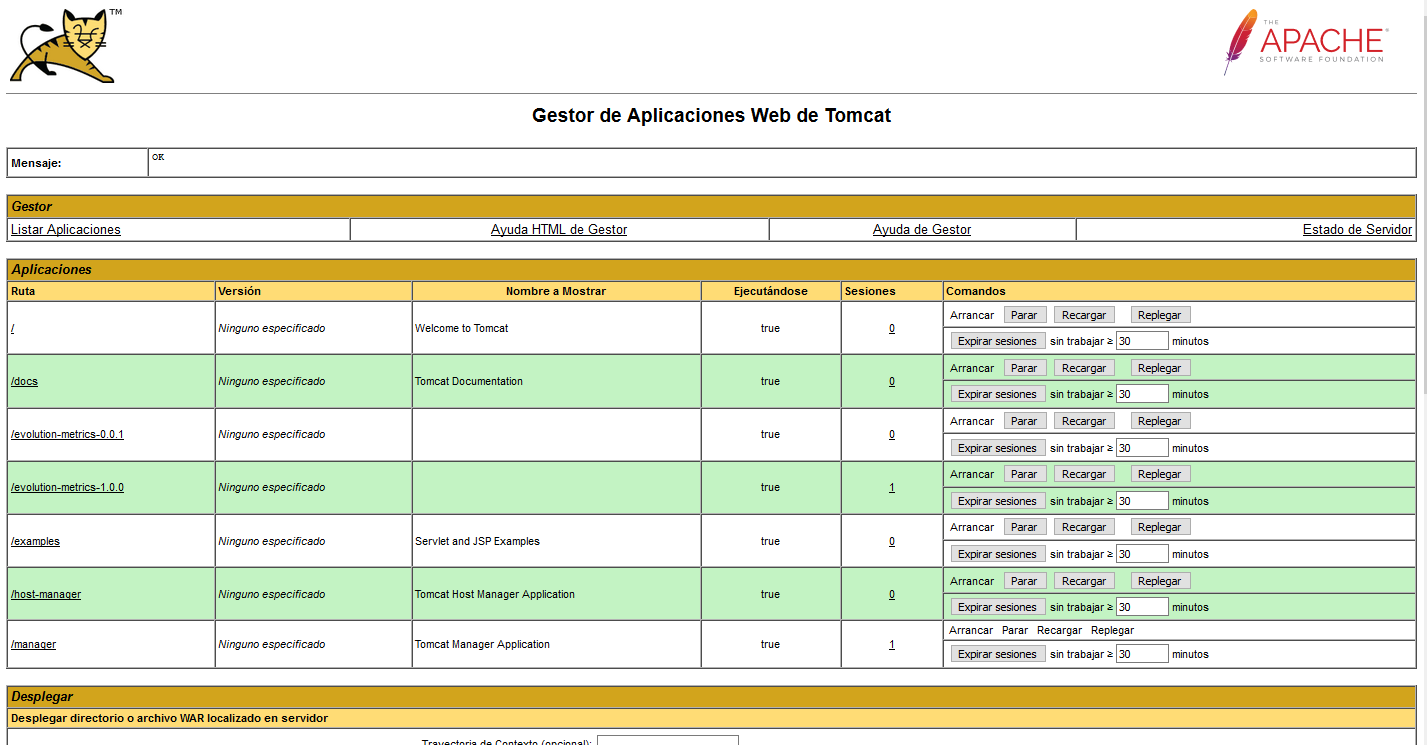
\includegraphics[scale=0.35]{M4_TomcatAppManager}
			\caption{Gestor de aplicaciones Tomcat con dos versiones desplegadas de la aplicación de este proyecto}\label{fig:M4_TomcatAppManager}
		\end{figure}
		\FloatBarrier
		
\end{description}
\subsection{Logging}
El \textit{logging} es el proceso que permite ver lo que ocurre durante la ejecución de la aplicación para poder depurar errores y analizar comportamientos para solucionar diferentes problemas. Este proceso es útil tanto en la fase de desarrollo del proyecto como en la de producción una vez la aplicación está desplegada y en uso por usuarios finales.

\begin{description}
	\item[SLF4J.] Visualización del \textit{logging}.
	Sirve como una simple fachada o abstracción para varios marcos de registro (por ejemplo, java.util.logging, logback, log4j) que permite al usuario final conectar el marco de registro deseado en el momento de la implementación.
	
		Enlace a página de descarga:
	
		\url{https://www.slf4j.org/download.html}
	
	\item[Log4j 2.] Logger. Se ha utilizado actualizado la versión a la 2.17.2 desde v2.11.2 utilizada por el proyecto previo \cite{TFGPrevio} para evitar diferentes vulnerabilidades.
	
	 	Enlace a página de descarga:
	
	 	\url{https://mvnrepository.com/artifact/org.apache.logging.log4j/log4j-core/2.17.2}\\
	
		SLF4J (\textit{Simple Logging Facade for Java}) es una capa intermedia entre el logger (\textit{java.util.logging}, \textit{logback}, \textit{log4j}, etc) y la aplicación, esto permite poder cambiar de logger fácilmente en tiempo de despliegue sin tener que realizar grandes cambios en el código de la aplicación.
		
		Esta herramienta permite configurar este proceso por medio de un fichero log4j2 con extensión XML, JSON, YAML o Properties\footnote{Manual de configuración de Log4j 2: \url{https://logging.apache.org/log4j/2.x/manual/configuration.html}} \cite{apache_apache_nodate}. En este proyecto se configuró mediante un fichero con extensión \textit{.properties}. 
		
		Ambas herramientas están integradas con Maven, y solo es necesario añadir en el fichero \ruta{pom.xml} las dependencias correspondientes.
	
\end{description}
\subsection{Pruebas}
La fase de pruebas permite comprobar que la implementación realizada funciona correctamente y no contiene errores. Se han implementado dos tipos de pruebas: unitarias y de integración. Las unitarias prueban los diferentes módulos y las de integración prueban la relación que tienen los diferentes módulos entre sí.
\begin{description}
	\item[JUnit5]. Conjunto de bibliotecas para el desarrollo de pruebas unitarias. 
	
		Se ha utilizado la versión  v5.3.1. Enlace a página de descarga:
		
		\url{https://junit.org/junit5/}
		
		JUnit permite realizar pruebas unitarias de forma automática o semiautomática de aplicaciones Java. Se han ejecutado de ambas formas en el proyecto. La automatización completa ha sido posible gracias a las herramientas de CI (\textit{Continuous Integration}) de Github \textit{GitHub Actions}: 
		\url{https://docs.github.com/es/actions}
		
		Esta versión de JUnit 5, sobre la anterior JUnit 4, ha influido en este proyecto de la siguiente manera:
		\begin{itemize}
			\item JUnit 5 soporta \textbf{Java 11}.
			
			\item Permite realizar asertos (\textit{asserts}) de tipo \textit{\textbf{assertAll()}} \footnote{\url{https://junit.org/junit5/docs/current/api/org/junit/jupiter/api/Assertions.html}}. Este tipo de asertos permite tratar varios asertos como una unidad. Se utilizaron en versiones anteriores de la aplicación, pero realmente no eran necesarios y se optó por quitarlos.
			
			\item Permite realizar \textbf{comprobaciones de lanzamiento de excepciones} en asertos del tipo \textit{assertThrows()}.
			
			\item Permite realizar suposiciones (\textit{\textbf{assumptions}}) que permiten realizar una comprobación que pasará por alto un test (lo marca como \textit{skipped}) si la comprobación falla. Es decir que no lo marcará como error, simplemente no realizará el test. 
			\\Esto ha sido útil de cara a probar funciones que realizan conexiones a GitLab o GitHub que requieren credenciales de acceso que no se pueden publicar en los test ya que quedarían publicadas. Por tanto estos test tienen presunciones que comprueban que se tiene las credenciales de acceso y no se realizan los test si no se dispone de estas credenciales, en lugar de lanzar un error por no poder realizar la conexión.
			\\Estos test se ejecutan manualmente por el programador en su equipo local y no se ejecutan automáticamente en el proceso de integración continua.
			
			\item Permite crear \textbf{test parametrizados}. Estos son test que prueban funciones que requieren argumentos. Cada combinación de argumentos es un caso de prueba, y crear un test para cada combinación es un caso claro del defecto de código: `código duplicado'. Por ello estos argumentos se pueden generar mediante funciones, enumeraciones, proveedores de argumentos o recolectar desde un CSV y solo ser necesario un test para todas las combinaciones de argumentos posibles.
		\end{itemize}
\end{description}
\subsection{Frameworks y librerías específicas para el proyecto}
%\todo Además de los enlaces de la aplicación añade los enlaces de tu repositorio
\begin{description}
	\item[gitlab4j-api]. Framework de conexión a GitLab API. 
	
		Se ha actualizado a última versión disponible, la versión  v4.19.0. Enlace:
		
		\url{https://javadoc.io/doc/org.gitlab4j/gitlab4j-api/4.19.0/index.html}
		
		
	\item[Apache Commons Math]. Librería que se utiliza para matemáticas descriptivas y que ha servido para el cálculo de cuartiles, necesarios para obtener los valores umbrales de las métricas según las estadísticas. 
	
		Se ha utilizado la versión  v3.6.1. Enlace a página de descarga:
	
		\url{https://commons.apache.org/proper/commons-math/download_math.cgi}
		
		Ejemplo de uso de la clase \textit{DescriptiveStatistics} de la librería:
		
\begin{minipage}{\linewidth}
{\tiny 
\begin{verbatim}[breaklines]
...
ArrayList<Double> datasetForMetric;
Double q1ForMetric, q3ForMetric;
DescriptiveStatistics descriptiveStatisticsForMetric;

descriptiveStatisticsForMetric = new DescriptiveStatistics(datasetForMetric
	  .stream()
	  .mapToDouble(x -> x)
	  .toArray());
q1ForMetric = descriptiveStatisticsForMetric.getPercentile(25);
q3ForMetric = descriptiveStatisticsForMetric.getPercentile(75);
...
\end{verbatim}
}
\end{minipage}		

\end{description}
\subsection{Interfaz gráfica}
\begin{description}
	\item[Vaadin]. Framework para desarrollo de interfaces Web con Java.
		Se ha utilizado la versión  v13.0.0 Enlace:
		
		\url{https://vaadin.com/}
		
		Con este framework no ha sido necesario escribir HTML, solo Java y CSS para los estilos. 
		\\Como ejemplo de esto, para implementar un \textit{input} se utilizaría el siguiente código:
		
\begin{minipage}{\linewidth}
\tiny \begin{verbatim}
...
EmailField emailField = new EmailField();
emailField.setLabel("Email address");
add(emailField);
...
\end{verbatim}
\end{minipage}	

		y el resultado sería el de las siguientes figuras Fig. \ref{fig:M4_Vaadin_Input_1} y Fig. \ref{fig:M4_Vaadin_Input_2}
\begin{figure}[!h]
	\centering
	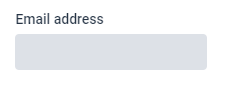
\includegraphics[scale=0.5]{M4_Vaadin_Input_1}
	\caption{Input generado por Vaadin vacío}\label{fig:M4_Vaadin_Input_1}
	
	
	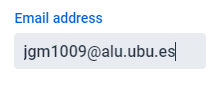
\includegraphics[scale=0.5]{M4_Vaadin_Input_2}
	\caption{Input generado por Vaadin con texto}\label{fig:M4_Vaadin_Input_2}
\end{figure}
\FloatBarrier

\end{description}
\subsection{Desarrollo y despliegue continuo}
\begin{description}
	\item[GitHub]. Forja (plataforma de desarrollo colaborativo) para alojar proyectos utilizando el sistema de control de versiones Git en la que se ha almacenado el proyecto en un repositorio Git.
	
		Enlace a GitHub:
		
		\url{https://github.com/}
		
		Enlace al repositorio del proyecto:
		
		\url{https://github.com/Joaquin-GM/GII_O_MA_19.07-Comparador-de-metricas-de-evolucion-en-repositorios-Software}
		
		En este proyecto se ha optado por utilizar GitHub frente a la primera iteración del proyecto \cite{TFGPrevio} para explorar su funcionalidad y comprobar que también es utilizable. Para más información hay una comparativa entre GitHub y GitLab en la sección \ref{sect:3_2_1_GitHubVSGitLab}.
		
	\item[Codacy]. Herramienta de generación automática de informes de calidad de código.
	
		 Enlace a Codacy:
		 
		 \url{https://www.codacy.com/}
		 
		 Enlace a proyecto en Codacy: 
		 
		 % TODO -> cuando esté generado poner el enlace al manual del proyecto
		 \url{https://app.codacy.com}
	
	\item[JaCoCo]. Librería utilizada para generar informes de cobertura del código en Java. Estos informes se pueden mostrar en GitHub fácilmente publicando los informes con formato HTML. También se han enviado estos informes a Codacy para que controle la cobertura además de la calidad de código.
	
		Se ha actualizado al proyecto para usar la la versión v0.8.7. 
		
		Enlace:
		
		\url{https://www.eclemma.org/jacoco/}
		
		Enlace a informe de JaCoCo en HTML sobre la cobertura del proyecto:
		
		% TODO -> cuando esté generado el primer nuevo informe poner url
		% \url{}
	
	\item[Heroku]. Herramienta para despliegue continuo (CD).
	
		Enlace a herramienta:
		
		\url{https://id.heroku.com/login}
		
		Enlace a aplicación desplegada:
		
		% TODO -> cuando esté desplegada la aplicación a través de GitHub Actions poner url
		% \url{}
	
\end{description}
\subsection{Documentación}
\begin{description}
	\item[LaTeX]. Sistema de composición de textos.
		Enlace a herramienta:
		
		\url{https://www.latex-project.org/}
		
	\item[TeXMaker]. Entorno de desarrollo de documentos LaTeX.
	
		Enlace a herramienta:
		
		\url{https://www.xm1math.net/texmaker/}
	
	\item[Zotero]. Herramienta de gestión de fuentes bibliográficas.
		
		Enlace a herramienta:
		
		\url{https://www.zotero.org/}
	
\end{description}
\section{Técnicas}
\begin{itemize}
	\item A lo largo del proyecto se han utilizado diferentes patrones de diseño \cite{gamma_patrones_2002} como Singleton, Factory Method, Wrapper, Builder, Listener, etc.En los apéndices se puede encontrar más información al respecto.
	
	\item Para el motor de métricas se ha utilizado como base el framework propuesto en \textit{Soporte de Métricas con Independencia del Lenguaje para la Inferencia de Refactorizaciones} \cite{marticorena_sanchez_soporte_2005}. Ver Fig. \ref{fig:MCTMotorMetricas} en la sección \ref{sect:3_3_3_FrameworkMedicion}.
	
	\item El ciclo de vida del software de este proyecto se ha basado en \textit{Scrum}\cite{scrum_master_scrum_2019}, es decir, ha seguido un modelo de proceso iterativo e incremental. En el siguiente capítulo se puede encontrar más información sobre éste.
\end{itemize}
